\chapter{Methodology}
The research concept of the thesis is divided as follows: first, a systematic literature review (SLR) will be conducted according to \cite{HevnerAR2004DSiI, vomBrockeJan2019TDgs, Webster2002AnalyzingTP}. Second, Knowledge from the first part will be applied to the project RAPADO. The implementation part of this master thesis follows an agile development approach. RAPADO use cases for zero-knowledge proof protocols are investigated, conceptualized, and evaluated, considering aspects found in previously examined literature and preliminary work at the department of information systems at Freie Universit{\"a}t Berlin. The application of acquired technical and theoretical knowledge is at focus, while the use cases implemented can be exchanged in the future during further project research. 

\section{Systematic Literature Review}
The initial and current status and results of project RAPADO are reflected on. From this analysis, potential use cases and design requirements for the application of zero-knowledge proofs are derived. Following the requirement to accumulate knowledge within the project in order to build expertise in blockchain-based development for the aviation industry, the literature survey focuses on the design of zero-knowledge proofs and theoretical foundations. Opportunities and challenges are displayed by considering practical examples. The second part of the research concept is the implementation of a zero-knowledge application for the use case of MRO data attestation and verification, whereby the demonstration of technical mechanisms is at focus.

This master thesis is associated with preliminary work carried out within RAPADO at the department of information systems. Immediate previous research concludes with conceptual solutions and a decentralized application for aviation industry MRO documentation, centering storage and traceability \citep{ZedelJ}. Hereby, use cases of uploading, storing, and trading aircraft spare parts certificates were given and specific blockchain platform architectures were used. This research extends previous findings. However, it takes a new perspective by further investigating possible use cases for ZKP as methods of automating verification processes, preserving data confidentiality and suggesting suitable data formats. The results are expected to represent the broader research project, i.e., beyond previously used software.

The focus of the SLR are zero-knowledge proofs with the scope of classification, opportunities, challenges, evaluation methods, and examples in practice. The design of zero-knowledge proofs needs to be understood from a theoretical perspective. Application domains and use cases applicable to the research project are at focus, which excludes topics of cryptocurrencies and embedded systems. The objective of this survey is to provide an extensive overview on the design and implementation of zero knowledge proofs, as well as to bring out practical and critical implications within the domain of distributed ledger technology. The final search string is derived from a concept map (Figure \ref{fig:concept_map}) and the literature found is summarized through a concept matrix, with headers displayed in Figure \ref{fig:concept_matrix} and the entire matrix in Appendix \ref{Appendix A}.

\begin{figure}[hbt]
	\centering
		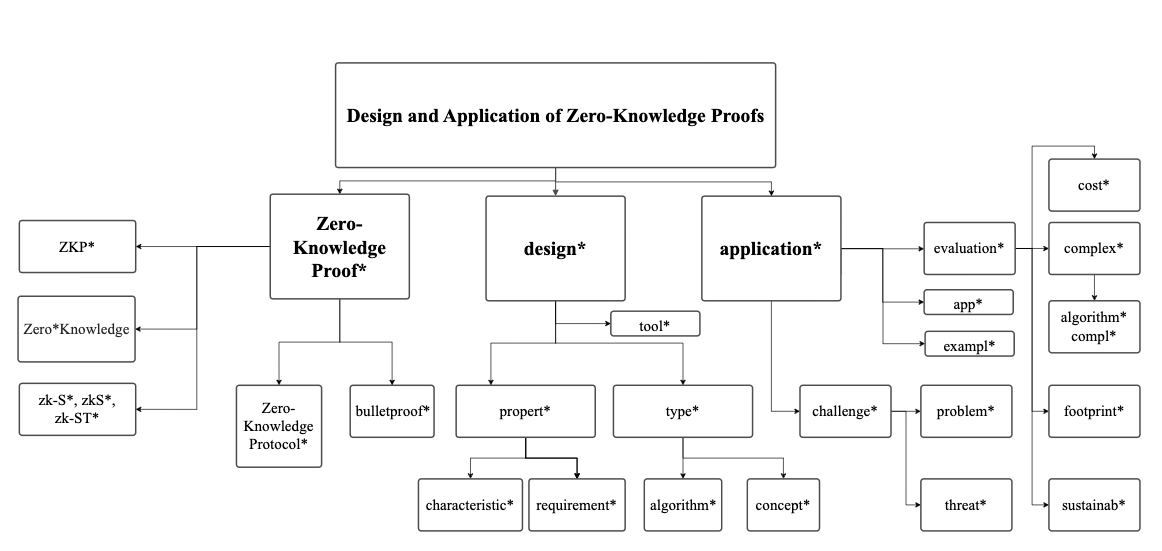
\includegraphics[width=0.99\textwidth]{Pictures/concept map.png}
	\caption{Search compression process}
	\label{fig:concept_map}
\end{figure}

The research question is assigned to topics of Computer Science, Mathematics, and Information Systems. For the search, the databases Web of Science (WoS), Association of Computing Machinery (ACM), zbMATH, arXiV, Association of Information Systems (AIS), and Institute of Electrical and Electronics Engineers (IEEE) were queried. Articles were searched in Title, Keywords, and Abstract, and if possible, with date restrictions back to 2018 (WoS) and 2006 (ACM). The following search string was used: (("ZKP*" OR "Zero-Knowledge*" OR "zero*knowledge*algorithm*" OR "zero*knowledge*protocol*" OR "zero*knowledge*proof*" OR "zkS*" OR "zk*SNA*" OR "zk*STA*" OR "zk*STO" OR "bulletproof*") AND ("application*" OR "example*" OR "app*") AND ("carbon*footprint*" OR "*complexity*" OR "evaluation*" OR "cost*" OR "sustainab*" OR "environment*") AND ("challenge*" OR "threat*" OR "problem*"). After deduplication, the search resulted in 580 hits, which were condensed according to the following approach. First, the result was filtered by English or German resources which have more than or equal to five citations with three times or higher past 180 days usage (560 hits). The next exclusion criteria were applied in Title and Keywords (396 hits), Abstract (319 hits), and Full-text (80 hits), of which backward/forward search added another 20 hits. 

\begin{figure}[hbt]
	\centering
		
\includegraphics[width=0.99\textwidth]{Pictures/bsp1.png}
	\caption{Concept Matrix}
	\label{fig:concept_matrix}
\end{figure}

Results of the survey can be summarized into the following topics. 
\begin{itemize}
    \item Algorithm design topics: Zero-knowledge proofs are designed by combining proof systems and cryptographic means to achieve specific characteristics. Proof systems are examined and defined, linking and presenting cryptographic tools within the scope of building zero-knowledge argument systems in the area of applicable blockchain-based solutions.
    \item Subsequent to the previous item, most widely used and performative zero-knowledge proofs are described in more detail, i.e., algorithms of specific zk-SNARKs, zk-STARKS, and Bulletproofs.
    \item Selective literature is summarized according to the following problem domains identified: Electronic Voting and Government, Electronic Auctions, Data Queries and Traceability, Electronic Healthcare, Cloud Security, and Scaling.
    \item Opportunities and challenges are summarized and aligned by evaluating and comparing the different algorithms qualitatively through literature review and quantitatively through complexity analysis.
\end{itemize}

\section{Implementation and Evaluation}
Results of this masters' thesis are three artifacts, each satisfying a requirement in project Rapado. The requirements are derived from previous work at the department of Information Systems at Freie Universit{\"a}t Berlin and workshops held within the project consortium. From these broader requirements, specific design requirements are extracted, which can be referred to during implementation. The development of artifacts is conducted in an agile and iterative manner, whereby the demonstration of the technical application of zero-knowledge proofs via prototyping is at focus \citep{mci/Wilde2007}. The following table describes the three artifacts and their implementation approach (Table \ref{tab:summary_artifacts}). 

The algorithms studied in chapter 5 are evaluated according to their complexity. Artifact 1 represents a reference document to understand zk-SNARKs functionalities. It is shown in the final state after recurring consultation between author and research department. Artifact 2 results from an agile implementation approach and is evaluated through first feedback collection from the project partner. Enhancements are implemented and summarized in chapter 6. Artifact 3 is evaluated by revisiting project and design requirements to assess current and future project needs. 

\setlength{\tabcolsep}{2ex}
\renewcommand{\arraystretch}{1.5}%
\begin{table}[htb]
	\centering
	    \caption{Results and Implementation Description}
		\begin{tabular}{|m{0.001\linewidth} | m{0.12\linewidth} | m{0.35\linewidth} | m{0.4\linewidth} |}
		\hline
		\textbf{}& \textbf{Artifact} & \textbf{Short Description} & \textbf{Implementation} \\ \hline
            1&Groth16 Example \newline Calculation & Step-wise computation of Groth16 protocol by taking a simple polynomial as example. The goal is to create a reference document to underline zk-SNARKs functionality, corresponding to the requirement of accumulating expertise on the topic within the project. & Developed during research phase on zk-SNARKs theory and functionality by taking a simple proof example and following the Groth16 protocol steps \citep{Groth2016OnTS}. \\  \hline
            2&zk-DApp MRO \newline Attestation & Zero-knowledge decentralized application to attest to MRO data of parts and create a trusted verified process. & Agile development with focus of demonstrating the functionality of plonk zk-SNARKs and practical implementation with circom and snarkjs. First feedback is collected and implemented. \\ \hline 
            3&Zero-Knowledge Data \newline Structure & Motivated by recurring comments during workshops and project consortium meetings, this is a first architecture prototype to enable further discussion of effective data formats and digitization of spare parts and corresponding documents. & Analyzing similar efforts in other alternative fields of research \citep{sedlemeirgrenenergy}, key insights are combined with results from the literature survey to implement first ideas and approaches to utilize zero-knowledge proofs to create effective data formats and standards for the future of aviation. \\  \hline 
	\end{tabular}
\label{tab:summary_artifacts}
\end{table}
\begin{comment}
-review of project requirements-->ableiten von design requirements
- with focus at technical functionalities, two use cases were picked out and developed in an agile manner, presenting very first prototypes for open discussion further in the project, main goal of knowledge accumulation is satisfied in chapter 5, designed and implemented artifacts satisfy two other main project requirements
- evaluation according to complexity analysis, fit to the project needs, limitations and future outlook
\end{comment}




\begin{comment}
SLR
Analysis of other resources
--> ends with requirements
(how good/bad the solution is)
-quantitative and qualitative evaluation, e.g. Laufzeit und Interviews 
- say what is not in scope
-DO NOT describe some agile method for the sake of having it! Just say it is a rather agile method etc.

I. Systematic literature review according to vom Brocke, Cooper and Webster: 
    1. Definition of Scope
        - classification, examples, challenges and evaluation methods of zero knowledge proof protocols 
        
    2. Conceptualization
        - work with concept map
        - derive at a search string
        
    3. Literature Search and Selection
        - look for review paper first to get good overview about the topic
        a) exclude paper that are too old and have too few citations and/or low impact factor (e.g. 5.5 is high)
        b) exclusion acc. to title and keywords
        c) exclusion acc. to abstract & structure of paper & RQ
        c) exclusion acc. to full text & availability of resource
        
    4. Synthesizing of Literature
        - cluster definitions, examples, drawbacks and evaluation methods (first suggestion can be found in the preliminary agenda)
        - write overview section about ZKP (Chapter 4)
- - - - - - -
How to know if a paper is useful for me?
1.title 2.keywords 3.abstract 4.structure of the paper 5.examples/use cases 6.research question/formal problem definition
- - - - - - -
% DSR muss nicht sein, kann auch SCRUM oder {"a}hnliches
II. Design Science Research
- DSR method acc. to Peffers and Hevner

\end{comment}
\begin{comment}
2) Ziel der Arbeit, scope of work
- not scope to practically integrate any of the concepts into existing DApp or any other existing system
- welche use cases gibt es f{"u}r ZKPs in RAPADO
- wie k{"o}nnte man diese Umsetzen

4) Ergebnisse skizzieren
- implementation can be a proof of concept, software artifact depends highly on complexity of the use case
\end{comment}